\documentclass{report}
\usepackage[utf8]{inputenc}
\usepackage[top=0cm, bottom=0cm, left=2cm, right=2cm]{geometry}
\usepackage[francais]{babel}
\usepackage[T1]{fontenc}
\usepackage{graphicx}
\usepackage{subcaption}


\begin{document}


\chapter{entreprise} 
	\section{biomedia (Imperial college, department of computing (biomedical image analysis section) )}
	\section{MIRTK}
	 => stable mais nécessite une maintenance et une amélioration continue pour rester pertinent
	 Intervention sur le module "Numerics", bibliotèque mathématique.
\chapter{ objectifs/cahiers des charges}
	\section{problématique (+contexte)}
	Arrayfire:Bibliothèque mathématique fournissant plusieurs fonctions de manipulation de matrices, ainsi que la possibilité de faire des boucles parallèles
	- Simplifier le code - Optimiser les performances de calcul -
	\section{cahier des charges}
	\section{objectifs et milestones}
	\subsection{Objectifs}- Ajouter ArrayFire à MIRTK, en remplaçant les fonctions d'EIGEN les moins adaptées par les fonctions d'AF
	- Garder la transparence
	- Supprimer er les TBB inutiles ou peu efficaces, et remplacer les autres par l'équivalent d'AF (gfor).
	\subsection{Diagramme de GANTT}
	 => gantt chart prévisionnel
	\begin{figure}[h!]
		\begin{center}
			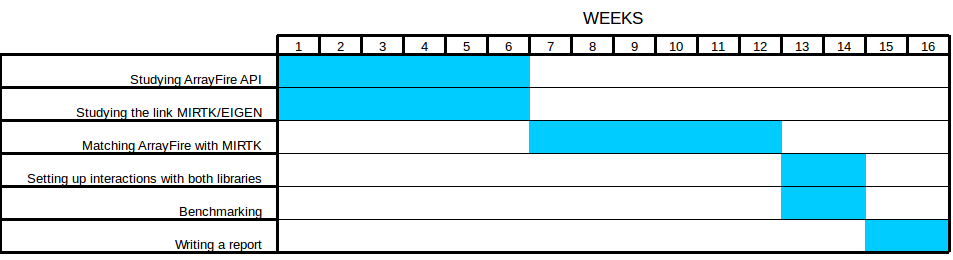
\includegraphics[width=18cm]{Reports/figures/estimated_gantt.png}
		\end{center}	
		\caption{Diagramme de GANTT prévisionnel}
		\label{Diagramme de GANTT prévisionnel}
	\end{figure}
\chapter{ réalisation}
	\section{profiling}
	Profiling => on identifie les fonctions sur lesquelles agir en premier
	On utilise Valgrind, qui, avec callgrind analyse la manière dont les caches sont utilisés, puis on double check avec VTune sur une autre machine.
	\section{integration d'arrayfire dans MIRTK}
	\section{benchmarking}
	 
	
\end{document}